\chapter{Análisis literario -- I}

\lettrine[lines=2,slope=.5em]{A}{ntonia tomó} el control del
teclado. Sus ojos relucían con un brillo que no podía explicarse
exclusivamente por el reflejo de la luz del monitor. Sus labios se
movían levemente, como si estuviera pronunciando internamente las
líneas que Cecilia acababa de escribir.

\begin{figure}[ht]
  \begin{minipage}[]{.5\textwidth}
    \begin{lstlisting}
$fn = 200;      
sphere(r=16);
translate([0,0,24])
  sphere(r=8);
translate([0,0,36])
  sphere(r=4);
translate([0,0,42])
  sphere(r=2);
translate([0,0,45])
  sphere(r=1);
translate([0,0,46.5])
  sphere(r=.5);
translate([0,0,47.25])
  sphere(r=.25);       
    \end{lstlisting}%$
  \end{minipage}\hfill
   \begin{minipage}[]{.5\textwidth}
     \centering
     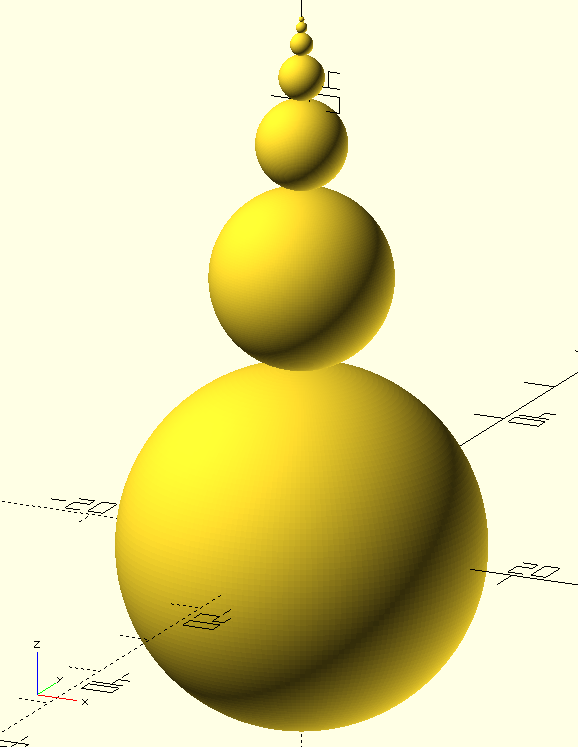
\includegraphics[width=.8\textwidth]{imagenes/esferas}
   \end{minipage}
%   \caption{Esferas apiladas por Cecilia en el capítulo anterior.}
  \label{fig:esferas-seis}
\end{figure}


\section{Expresiones matemáticas}

---Empecemos por las alturas: ¿Cómo elegiste los valores 24, 36, 42,
45, etc., en la coordenada \coord{Z} de los \lstinline!translate!s?
---pre\-gun\-tó Antonia con una sonrisa.

Cecilia miró atentamente a su amiga; por un momento cruzó por su mente
la posibilidad de que estuviera jugando con ella. Pero aun así decidió
contestar:


 \begin{figure}[ht]
   \centering
   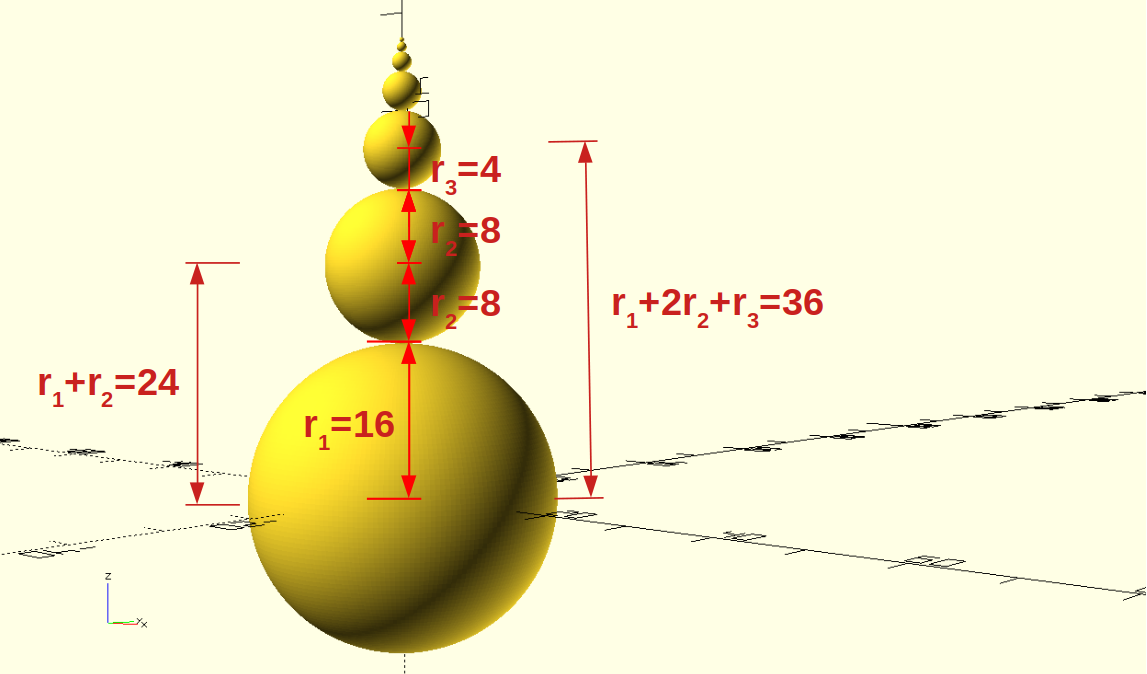
\includegraphics[width=.85\textwidth]{imagenes/esferas-anotadas}   
   \caption{Cálculos explícitos hechos por Cecilia para apilar esferas
     de radios decrecientes.}
   \label{fig:esferas-anotadas}
 \end{figure}


 ---La primera esfera, centrada en el origen, es de radio 16. La
 segunda, de radio 8, quería que fuera tangente a la primera. Luego,
 la altura de su centro debería ser igual a la suma de ambos radios:
 24. La tercera esfera era de radio 4: por lo tanto, la altura de su
 centro (a fin de resultar tangente a la segunda) debía igualar la
 suma de su radio, el radio de la primera y dos veces el radio de la
 segunda. El razonamiento se repite para las demás.

 Cecilia, tras concluir su explicación, en la que empleó un tono
 deliberadamente lento, volvió a mirar atentamente a Antonia a fin de
 comprobar en su gesto si había habido alguna intención juguetona en
 su pregunta inicial. Pero como su amiga mantenía la misma sonrisa
 franca que manifestaba cuando un asunto despertaba su interés,
 Cecilia decidió abandonarse a sus preguntas, ya sin temores.

 ---Entiendo la lógica, pero ¿por qué hiciste las cuentas vos? ¡A las
 computadoras les encanta hacer cuentas! Mirá ---dijo Antonia, y sus
 dedos sacaron vibrantes sonidos al teclado mientras modificaba las
 líneas de Cecilia:
 
\begin{lstlisting}
$fn = 200;      
sphere(r=16);
translate([0,0,16+8])
  sphere(r=8);
translate([0,0,16+2*8+4])
  sphere(r=4);
translate([0,0,16+2*8+2*4+2])
  sphere(r=2);
translate([0,0,16+2*8+2*4+2*2+1])
  sphere(r=1);
translate([0,0,16+2*8+2*4+2*2+2*1+.5])
  sphere(r=.5);
translate([0,0,16+2*8+2*4+2*2+2*1+2*.5+.25])
  sphere(r=.25);      
\end{lstlisting}%$


A Cecilia le pareció muy conveniente enterarse de que \openscad{}
aceptaba las operaciones matemáticas básicas como modo de expresión,
pero sinceramente no veía cómo eso mejoraba su texto.

---Lo que quería era mostrarte cómo \openscad{} acepta las operaciones
matemáticas básicas como modo de expresión ---confirmó Antonia, como
si leyera su mente palabra por palabra---. En este caso particular,
admito que no mejora sensiblemente tu texto; sin embargo, explicitar
las operaciones matemáticas puede sugerirnos ideas, realzando el
patrón que se encuentra detrás de ellas.

Antonia hizo un silencio que pudo parecer teatral, pero no lo fue:
volvió a sumergirse en el texto de Cecilia para indagar en él una
nueva reescritura.

 \section{Variables}

 ---Claramente, los radios de las esferas están firmemente vinculados:
 a partir de la primera, las demás tienen un tamaño igual a la mitad
 de la anterior. Si vos decidieras construir otra torre de esferas a
 partir de una inicial con radio diferente, deberías modificar las
 doce líneas de texto, cuando en realidad debería bastar (desde el
 punto de vista de la lógica de la construcción de la torre) con
 cambiar un solo dato: el radio de la primera esfera ---razonó
 Antonia, y a Cecilia no le costó nada estar de acuerdo.

 \guillemotright Para eso existen las \emph{variables}: `etiquetas'
 que representan un valor, por ejemplo numérico. Mirá ---dijo Antonia,
 mientras volvía a hacer tamborilear el teclado:


\begin{lstlisting}
$fn = 200;
radio = 16;

sphere(r=radio);
translate([0,0,radio+radio/2])
  sphere(r=radio/2);
translate([0,0,radio+2*radio/2+radio/4])
  sphere(r=radio/4);
translate([0,0,radio+2*radio/2+2*radio/4+radio/8])
  sphere(r=radio/8);
[...]
\end{lstlisting}%$

\guillemotright Una vez que definís la variable \texttt{radio}, cada
aparición de la misma en el texto es reemplazada por su valor; en
nuestro caso, 16.
 
Cecilia, una vez más y atraída ahora por un nuevo concepto que sentía
suavemente que le abría posibilidades que apenas podía sospechar por
el momento, entrecerró los ojos y se inclinó hacia el monitor, mientras
leía y asentía ligeramente con la cabeza.

---Está bueno ---susurró.

\section{En busca de una ley}

---¿No es cierto? ---asintió Antonia con una enorme sonrisa de
satisfacción---. Ahora, si cambiás de idea acerca del tamaño de la
base de la torre sólo debés modificar la línea número 2.

Tras un breve instante, en el que volvió a considerar el texto recién
modificado, continuó:

---Sin embargo, aún se puede mejorar. Como ya dijimos, el radio y la
altura de cada esfera están determinados por el radio de la primera;
lo único que resta decidir por nuestra parte es cuántas esferas
queremos. A partir de ahí, es pura mecánica: escribir las respectivas
líneas de texto cuidando de respetar la lógica matemática que hay
detrás de esa configuración en torre. Pero, ¿no son las computadoras
ideales para el trabajo mecánico y repetitivo? ¿Y qué pasa si querés
enhebrar, digamos, 25 esferas? ¿Será posible que debamos escribir 50
líneas de código virtualmente repetido? Es más, ¿no es sumamente
probable que una escritora se equivoque al escribir tediosas líneas de
contorno prácticamente idéntico?  Las computadoras, por otra parte, no
se distraen ni cometen erratas.

Antonia se detuvo, pensando evidentemente que su discurso no podía
tener más que una sola conclusión. Cecilia sintió que debía decir
algo, pero sólo acertó a levantar las cejas, invitándola a seguir.

---Pues bien ---prosiguió Antonia, un tanto contrariada por no haber
logrado el efecto buscado---; para lograr que la computadora realice
por su cuenta la columna de esferas deseada debemos buscar antes la
ley matemática que la sintetiza. Y para eso, una vez más, a mí me
sirve mucho reescribir las respectivas expresiones.


    \begin{lstlisting}
$fn = 200;
radio = 16;

translate([0,0,radio*0])
  sphere(r=radio/1);
translate([0,0,radio*3/2])
  sphere(r=radio/2);
translate([0,0,radio*9/4])
  sphere(r=radio/4);
translate([0,0,radio*21/8])
  sphere(r=radio/8);
translate([0,0,radio*45/16])
  sphere(r=radio/16);
[...]
\end{lstlisting}%$



Cecilia se irguió de golpe en su silla:

---¡Hey! ¿Qué hiciste? ---preguntó.

---Saqué factor común para cada altura ---contestó Antonia,
sorprendida---: \lstinline!radio+2*radio/2+radio/4! es igual a
\lstinline!radio*9/4!, ¿no?

---Sí, sí, claro ---Cecilia se ruborizó ligeramente---.  Pero también
agregaste al principio una traslación nula:
\lstinline!translate ([0, 0, radio*0])!. No sólo eso: al radio de la
primera esfera lo dividiste por 1:
\lstinline!sphere(r=radio/1)!... ¿Qué sentido tiene todo eso?

---Tiene muchísimo sentido ---se defendió Antonia---.  Estamos
buscando un patrón matemático que abarque a \emph{todas} las esferas,
y eso incluye a la primera.

 Cecilia asintió, comprendiendo, y trató de seguir el hilo de
 pensamiento propuesto por Antonia:

 ---La progresión de los radios es obvia: caen según potencias de 2:
 1, 2, 4, 8, 16, etc. ---afirmó.

 ---¡Tal cual! ---asintió Antonia---. Y las potencias de 2 pueden
 escribirse como $2^i$, donde $i$ es la posición en la progresión,
 siempre y cuando empecemos a contar desde 0. Así, el primer radio es
 igual a $\frac{\text{radio}}{2^0}$, ya que $2^0=1$.

---¡Qué conveniente que cualquier número elevado a la 0 sea
   igual a 1..! ---acotó Cecilia con una sonrisa, y las dos rieron
 ligeramente recordando sus tiempos de estudiantes, cuando pocos
 profesores les explicaban la razón profunda de esa ``rareza''.

 ---Muy bien ---prosiguió Antonia---; ya resolvimos los radios.
 Ataquemos ahora las alturas. La sucesión tiene esta pinta:
 radio$\times0$, radio$\times\frac{3}{2}$, radio$\times\frac{9}{4}$,
 radio$\times\frac{21}{8}$, radio$\times\frac{45}{16}$...

---Los denominadores son fáciles... ---se adelantó Cecilia.

---Tal cual ---confirmó Antonia---; más de lo mismo. Pero los
numeradores no son tan obvios.

---¡Múltiplos de 3! ---aventuró Cecilia---: $3\times 0$, $3\times 1$,
$3\times 3$, $3\times 7$, $3\times 15$...

---¡Exacto! ---exclamó Antonia---. ¿Y qué onda esos factores que
multiplican a 3: 0, 1, 3, 7, 15...?

Cecilia y Antonia estuvieron mirando la serie concentradas, hasta que
la primera disparó:

---¡Son una unidad menos que los téminos de la sucesión de las
potencias de 2!: $0=2^0-1$, $1=2^1-1$, $3=2^2-1$, $7=2^3-1$,
$15=2^4-1$,... ¡Las potencias de 2 nos persiguen!

Las dos rieron de buena gana, no sabemos si por la gracia del chiste
ñoño o por la alegría de sentir que resolvieron el secreto que una
progresión de esferas enhebradas guardaba tan celosamente.

---Pasando en limpio, entonces ---sentenció Antonia---; las alturas de
las esferas siguen la ley
$\frac{\text{radio}\times 3\times (2^i-1)}{2^i}$, donde $i$ representa
la ubicación de cada una en la sucesión, contando desde 0, y
\texttt{radio} es el radio de la primera esfera.

---Y los radios respetan esta otra ley: $\frac{\text{radio}}{2^i}$
---agregó Cecilia, satisfecha.\footnote{En rigor, lo que Cecilia y
  Antonia hallaron es una regularidad manifestada en unos pocos
  téminos; no están justificadas para extender su aplicación a
  cualquier valor de $i$. Sin embargo, considero que dicha regularidad
  es bastante convincente en sí misma, por lo que estimo que podemos
  confiar en ella.}$^,$\footnote{La confianza no reemplaza a un
  teorema; esas fórmulas deben ser demostradas matemáticamente antes
  de ser aplicadas, para no hablar de publicarse en un libro, aun
  cuando se trate de uno tan ínfimo como éste. (Nota del
  Editor)}$^,$\footnote{\Tongey (Nota de Cecilia, Antonia y Luis)}

 
---Y por hoy ya adelantamos mucho, Cecilia ---soltó Antonia con un
suspiro---. Creo que es mejor que sigamos en el capítulo siguiente,
donde aprovecharemos estas flamantes leyes para que la computadora
escriba por nosotras el texto completo de la torre.

Cecilia se preguntó a qué se refería Antonia con ``el capítulo
siguiente'', pero estaba demasiado entusiasmada y cansada como para
preguntar.



%%% Local Variables:
%%% mode: latex
%%% TeX-master: "../libro"
%%% End:
